\documentclass[brazil,dissertacao,epusp]{usp}
\usepackage[T1]{fontenc}  %Orienta a saída do texto a reproduzir caracteres especiais
\usepackage[utf8]{inputenc} %Permite que o usuário redija o documento utilizando caracteres especiais UTF-8

\usepackage{graphicx}  %Pacote de gerenciamento de figuras. Padrão para qualquer documento em LaTeX
\usepackage{helvet}  %Define Helvetica como fonte Sans Serif padrão
\usepackage{fancyvrb}  %Serve, por exemplo para aplicar estilos de texto individuais em trechos do texto
\usepackage{babel}  %Pacote de idioma
\usepackage{textcomp}  %Graças a esse pacote eu não preciso me preocupar com o símbolo °
%\usepackage{textgreek} %Define comandos para chamar letras gregas. Passei a usar o modo matemático pra isso.
%\usepackage{fixltx2e}  %Define \textsubscript{}, por exemplo.
\usepackage[font=normalsize]{subfig}  %Habilita utilização de subfiguras nos campos de figuras.
\usepackage{indentfirst}  %Faz a primeira linha após o chapter head ser indentada (vide definição de \thickline abaixo)
\usepackage{array}  %Graças a ele eu consigo editar elementos de tabela.
\usepackage{amsmath}  %Pacote com complementos do modo matemático.
\usepackage[symbolgreek]{mathastext}  %Equações ficam na mesma fonte do texto graças a isso. http://jf.burnol.free.fr/v13/mathastext.pdf
%\usepackage{paralist}  %Possibilita a criação de listas (ambiente enumerate) "inline".
\usepackage[hang,flushmargin]{footmisc}  %Deixa a indentação do rodapé do jeito que eu quero (vide exemplos no texto).
\usepackage{enumerate}  %Formata rótulos de listas enumeradas

\usepackage{siunitx}  %Formatação grandezas sistema internacional
\sisetup{output-decimal-marker={,}}

\usepackage{multirow}  %Multi colunas e multi linhas em tabelas

\usepackage{chemformula}

\makeatletter
%%%Define linhas horizontais (\thickline) e verticais (') para tabelas
\newcommand{\thickhline}{
  \noalign {\ifnum 0=`}\fi \hrule height 1.5pt
  \futurelet \reserved@a \@xhline
}
\newcolumntype{'}{@{\hskip\tabcolsep\vrule width 1.5pt\hskip\tabcolsep}}
\makeatother

\begin{document}
\bibliographystyle{usp}

\autor{Paula Arantes Ribeiro}
\orientador{Hélio Goldenstein}
\coorientador{Arthur Seiji Nishikawa}
\titulo{Método de aprendizado de máquina para previsão de pontos críticos de equilíbrio em ligas multi-componente}

% \agradecimentos{}

\resumo{
  Eu sou um TCC diva!
}
\palavrachave{Termodinâmica, Temperaturas críticas, Aprendizado de máquina, Redes neurais}

\resumole{}
\palavrachavele{Termodinâmica, Temperaturas críticas, Aprendizado de máquina, Redes neurais}

\programa{ep-metalurgica}
\departamento{ep-pmt}

\elementospretextuais  %Comando do USPTeX para criação dos elemenos pré-textuais do documento

\setlength\parindent{.85cm}  %Define em 0,85cm a identação da primeira linha do parágrafo.

\chapter{Introdução}

\chapter{Objetivos}

\chapter{Revisão bibliográfica}

\section{Os componentes do aço}

Aços podem ser vistos como uma combinação de ferro, carbono, manganês e outros elementos de liga. São conhecidas inúmeras combinações de ligas de ferro e carbono e, embora seja esperado que o aço tenha alta dureza e resistência, ele deve ser maleável a certas temperaturas \cite{Dossett2006}. Tal mudança de propriedades está relacionada com as diferentes estruturas do ferro e fases que o aço pode assumir.

O ferro em estado sólido tem duas formas alotrópicas, ou seja, diferentes estruturas cristalinas que dependem da temperatura e pressão. A baixas temperaturas, o ferro assume a estrutura cúbica de corpo centrado (CCC) e é denominado $\alpha$-Fe, ou ferrita; acima de 910°C, os cristais transformam sua estrutura para cúbica de faces centradas (CFC), também chamada de $\gamma$-Fe, ou austenita, de caráter paramagnético; sua estabilidade vai até 1400°C, onde volta a assumir uma estrutura CCC, mas chamada de $\delta$-Fe para diferenciar a faixa de temperatura de ocorrência.  Uma quarta estrutura que o ferro pode assumir é o $\beta$-Fe, a 770°C, quando a rede perde suas propriedades ferromagnéticas \cite{Totten2006}.

A partir da combinação dessas possíveis estruturas do ferro com outros elementos formam-se as ligas, geralmente no estado fundido. Como o ferro é a base do aço e tem estruturas cristalinas limitadas, é a sua combinação com outros átomos que resulta em diferentes propriedades. O carbono é insolúvel na fase $\alpha$, mas bastante solúvel na fase $\gamma$, pois a estrutura CFC permite a alocação dos átomos de carbono em seus interstícios. A presença do carbono diminui as temperaturas necessárias para que a liga de ferro sofra transformações de fases.

A porção de uma liga com estrutura e propriedades homogêneas é denominada fase. Em equilíbrio termodinâmico, as combinações entre o carbono e o ferro podem resultar em ferrita, austenita ou grafita, cujas relações com a temperatura e composição são mostradas no diagrama de equilíbrio da Figura \ref{fig:diagrama_fe-c}. Nessas condições, os constituintes do sistema Fe-C à temperatura ambiente seriam ferrita $\alpha$ e grafita.

\begin{figure}[ht!]
  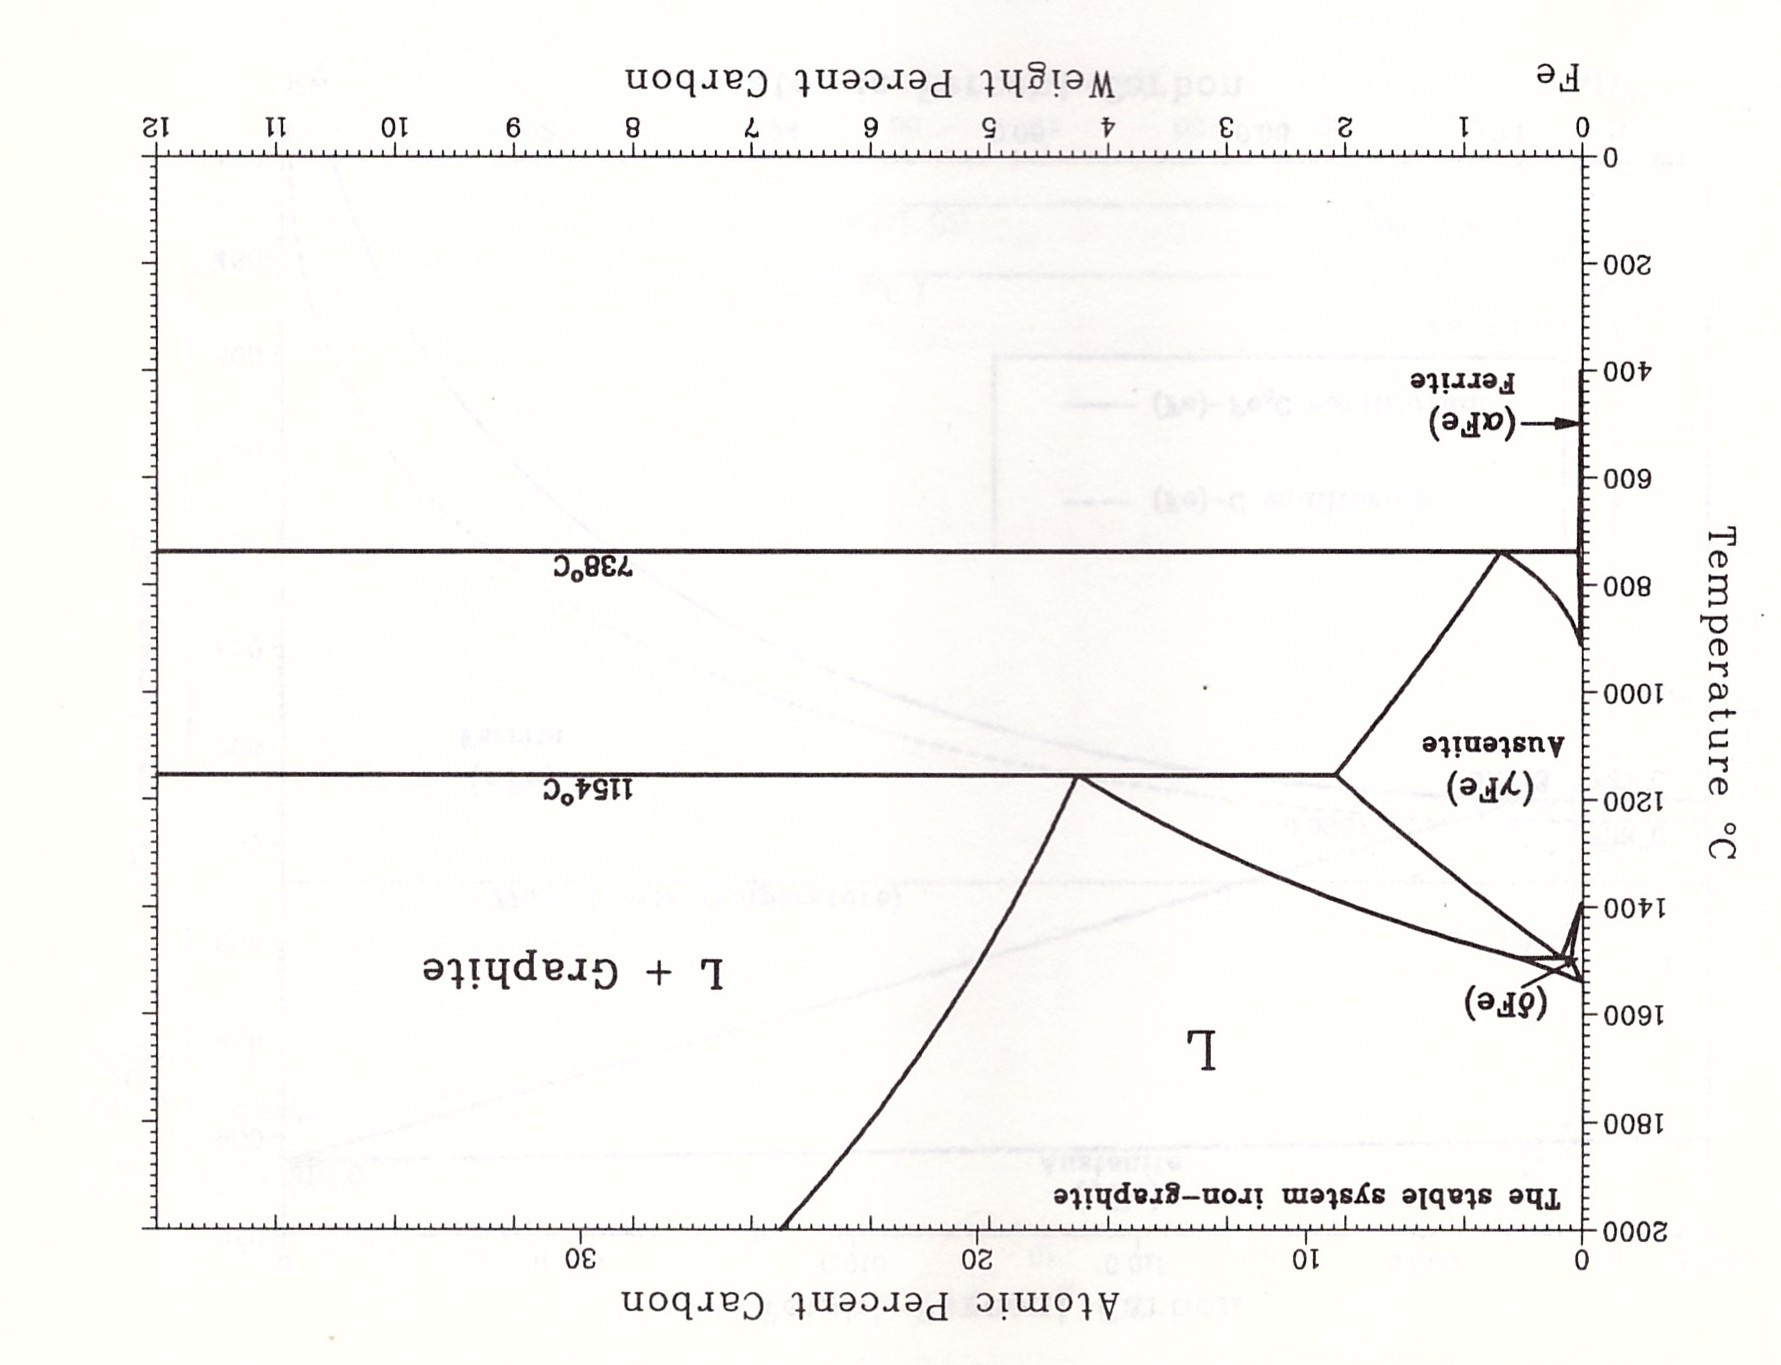
\includegraphics[width=.7\textwidth,angle=180]{img/Fe-C.jpg}
  \caption{Diagrama de equilíbrio ferro-carbono \cite{Massalski1996v1}}
  \label{fig:diagrama_fe-c}
\end{figure}

Entretanto a condição de equilíbrio não é verificada na produção industrial, uma vez que a solidificação e resfriamento do aço são muito rápidos. Assim, em vez de grafita forma-se carboneto de ferro, também chamado de cementita, que apesar de ser uma fase metaestável pode ser considerada estável, pois o coeficiente de difusão do carbono no ferro é muito baixo (\SI{2,9e-19}{cm^2/s}). Para essas condições, o diagrama de fase, que não pode ser chamado de diagrama de equilíbrio, é dado pela Figura \ref{fig:diagrama_fe-c_meta}.

\begin{figure}[ht!]
  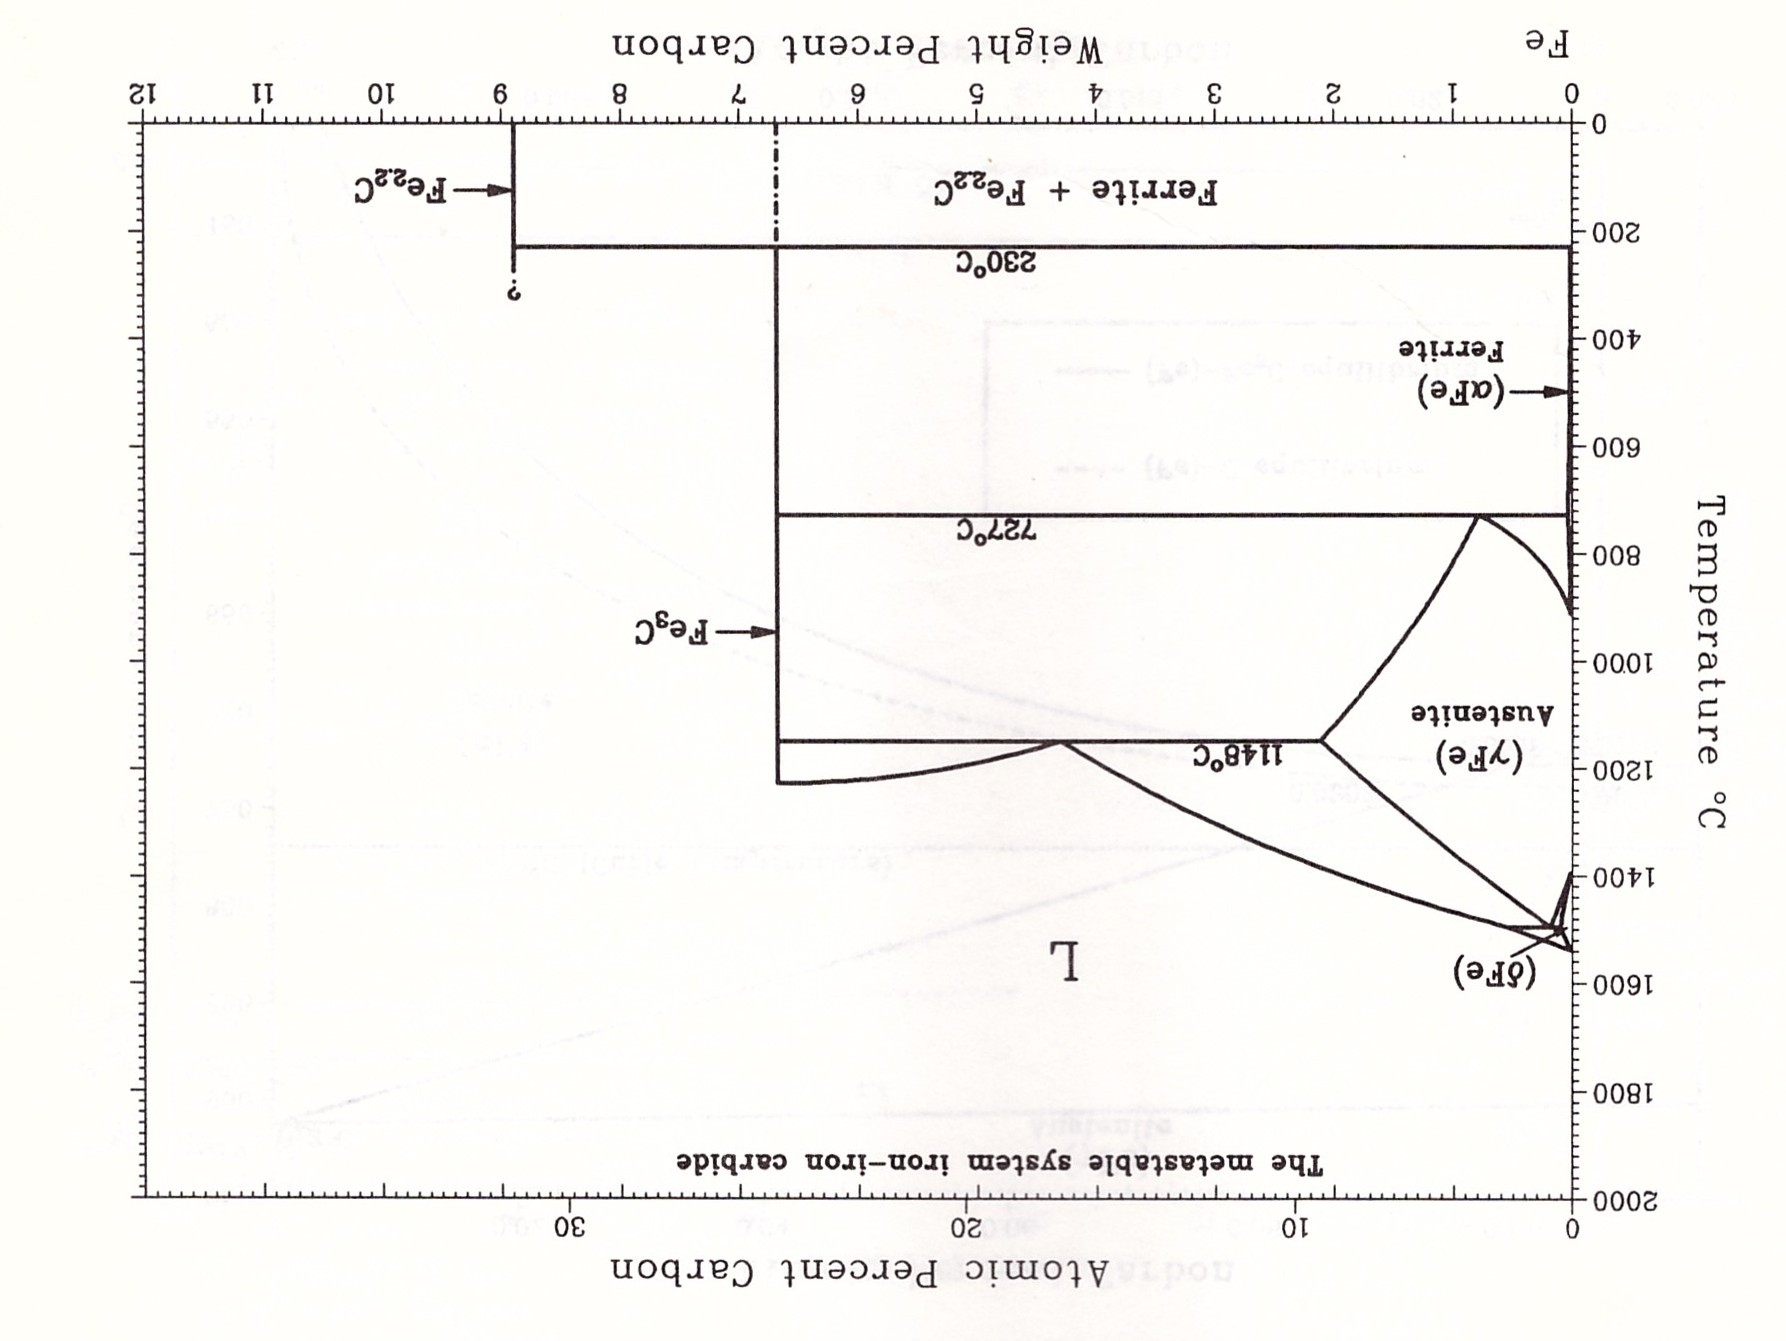
\includegraphics[width=.7\textwidth,angle=180]{img/Fe-C_meta.jpg}
  \caption{Diagrama de fases metaestável ferro-carbono \cite{Massalski1996v1}}
  \label{fig:diagrama_fe-c_meta}
\end{figure}

Um ponto importante do diagrama é o ponto eutetóide, no qual as três fases coexistem. Para um sistema apenas ferro e carbono, ele corresponde a aproximadamente 0,8\% C em massa. Assim, aços de composição abaixo desse ponto são denominados hipoeutetóides e, acima, hipereutetóides.

\section{Temperaturas cr\'iticas de aços}
Além das fases existentes no aço, existem temperaturas de transformação de extrema importância prática. O francês Le Chatelier foi o primeiro a atribuir a letra A para essas temperaturas, devido à palavra \textit{Arrêt}, que representa a parada na temperatura durante a transformação de fase \cite{Silva2010}.

Para exemplificar essas temperaturas críticas de transformação, utilizou-se dados de chamadas do software Thermo-Calc\textregistered{} para traçar o diagrama Fe-C metaestável para um aço 1\% Mn, em massa, da Figura \ref{fig:fe-1mn-C_isopleth}, bem como os gráficos de fração molar de fase em função da temperatura para aços hipo, hiper e eutetóide, das Figuras \ref{fig:fe-01c-1mn}, \ref{fig:fe-0727c-1mn} e \ref{fig:fe-1c-1mn} a seguir.

\begin{figure}[ht!]
  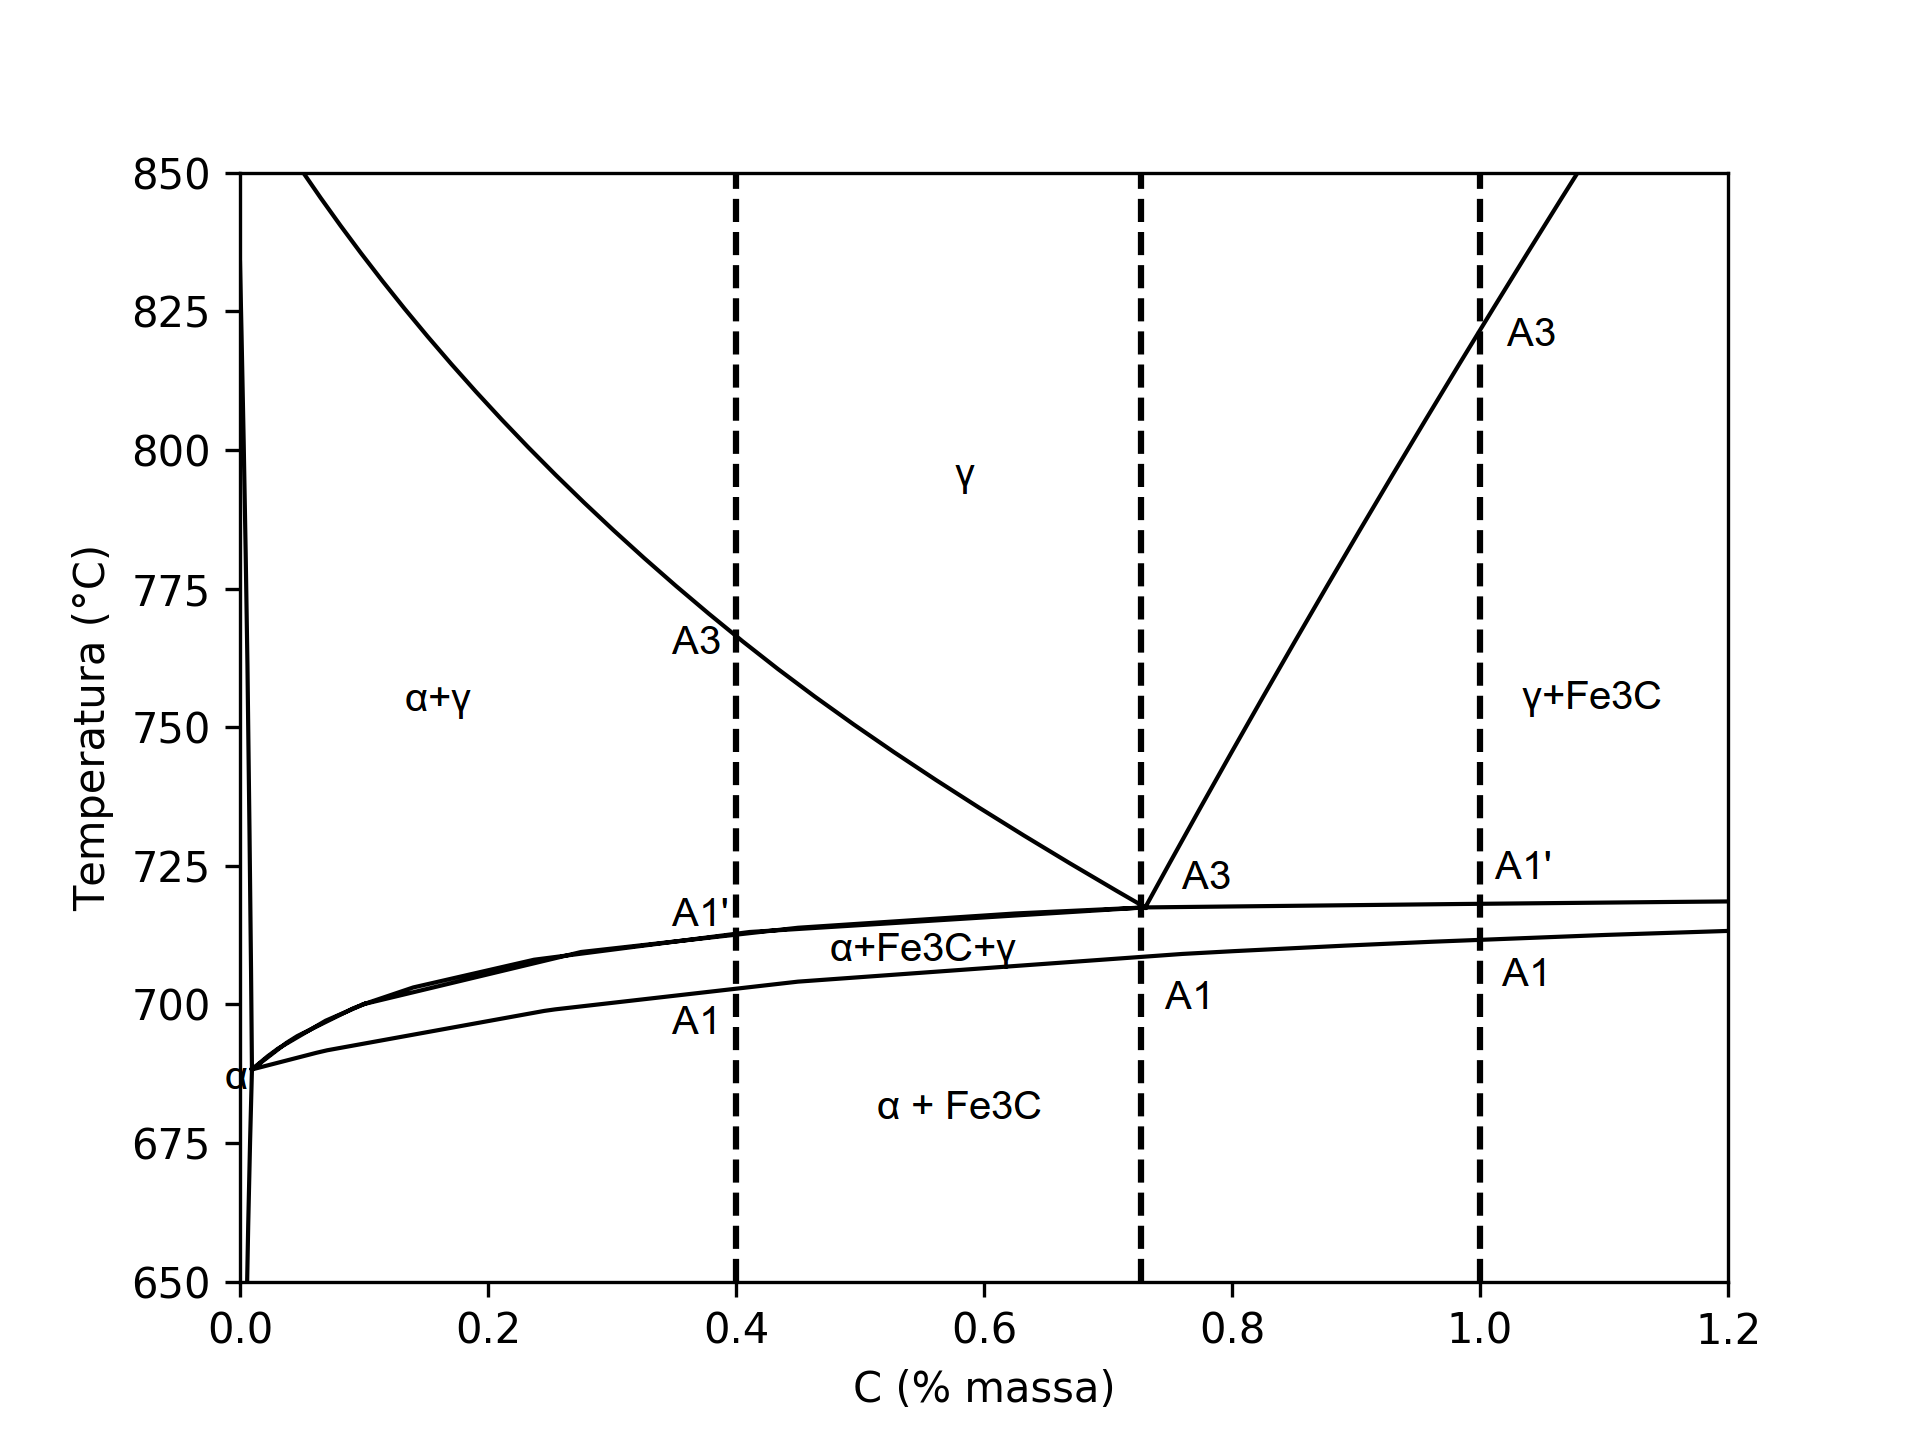
\includegraphics[width=.7\textwidth]{img/Fe-1Mn-C_isopleth_edited.png}
  \caption{Diagrama de fases Fe-C para aço 1\% Mn, em massa}
  \label{fig:fe-1mn-C_isopleth}
\end{figure}

A primeira linha vertical tracejada da Figura \ref{fig:fe-1mn-C_isopleth} representa um aço hipoeutetóide e sua fração molar de fases pode ser vista na Figura \ref{fig:fe-01c-1mn}.

\begin{figure}[ht!]
  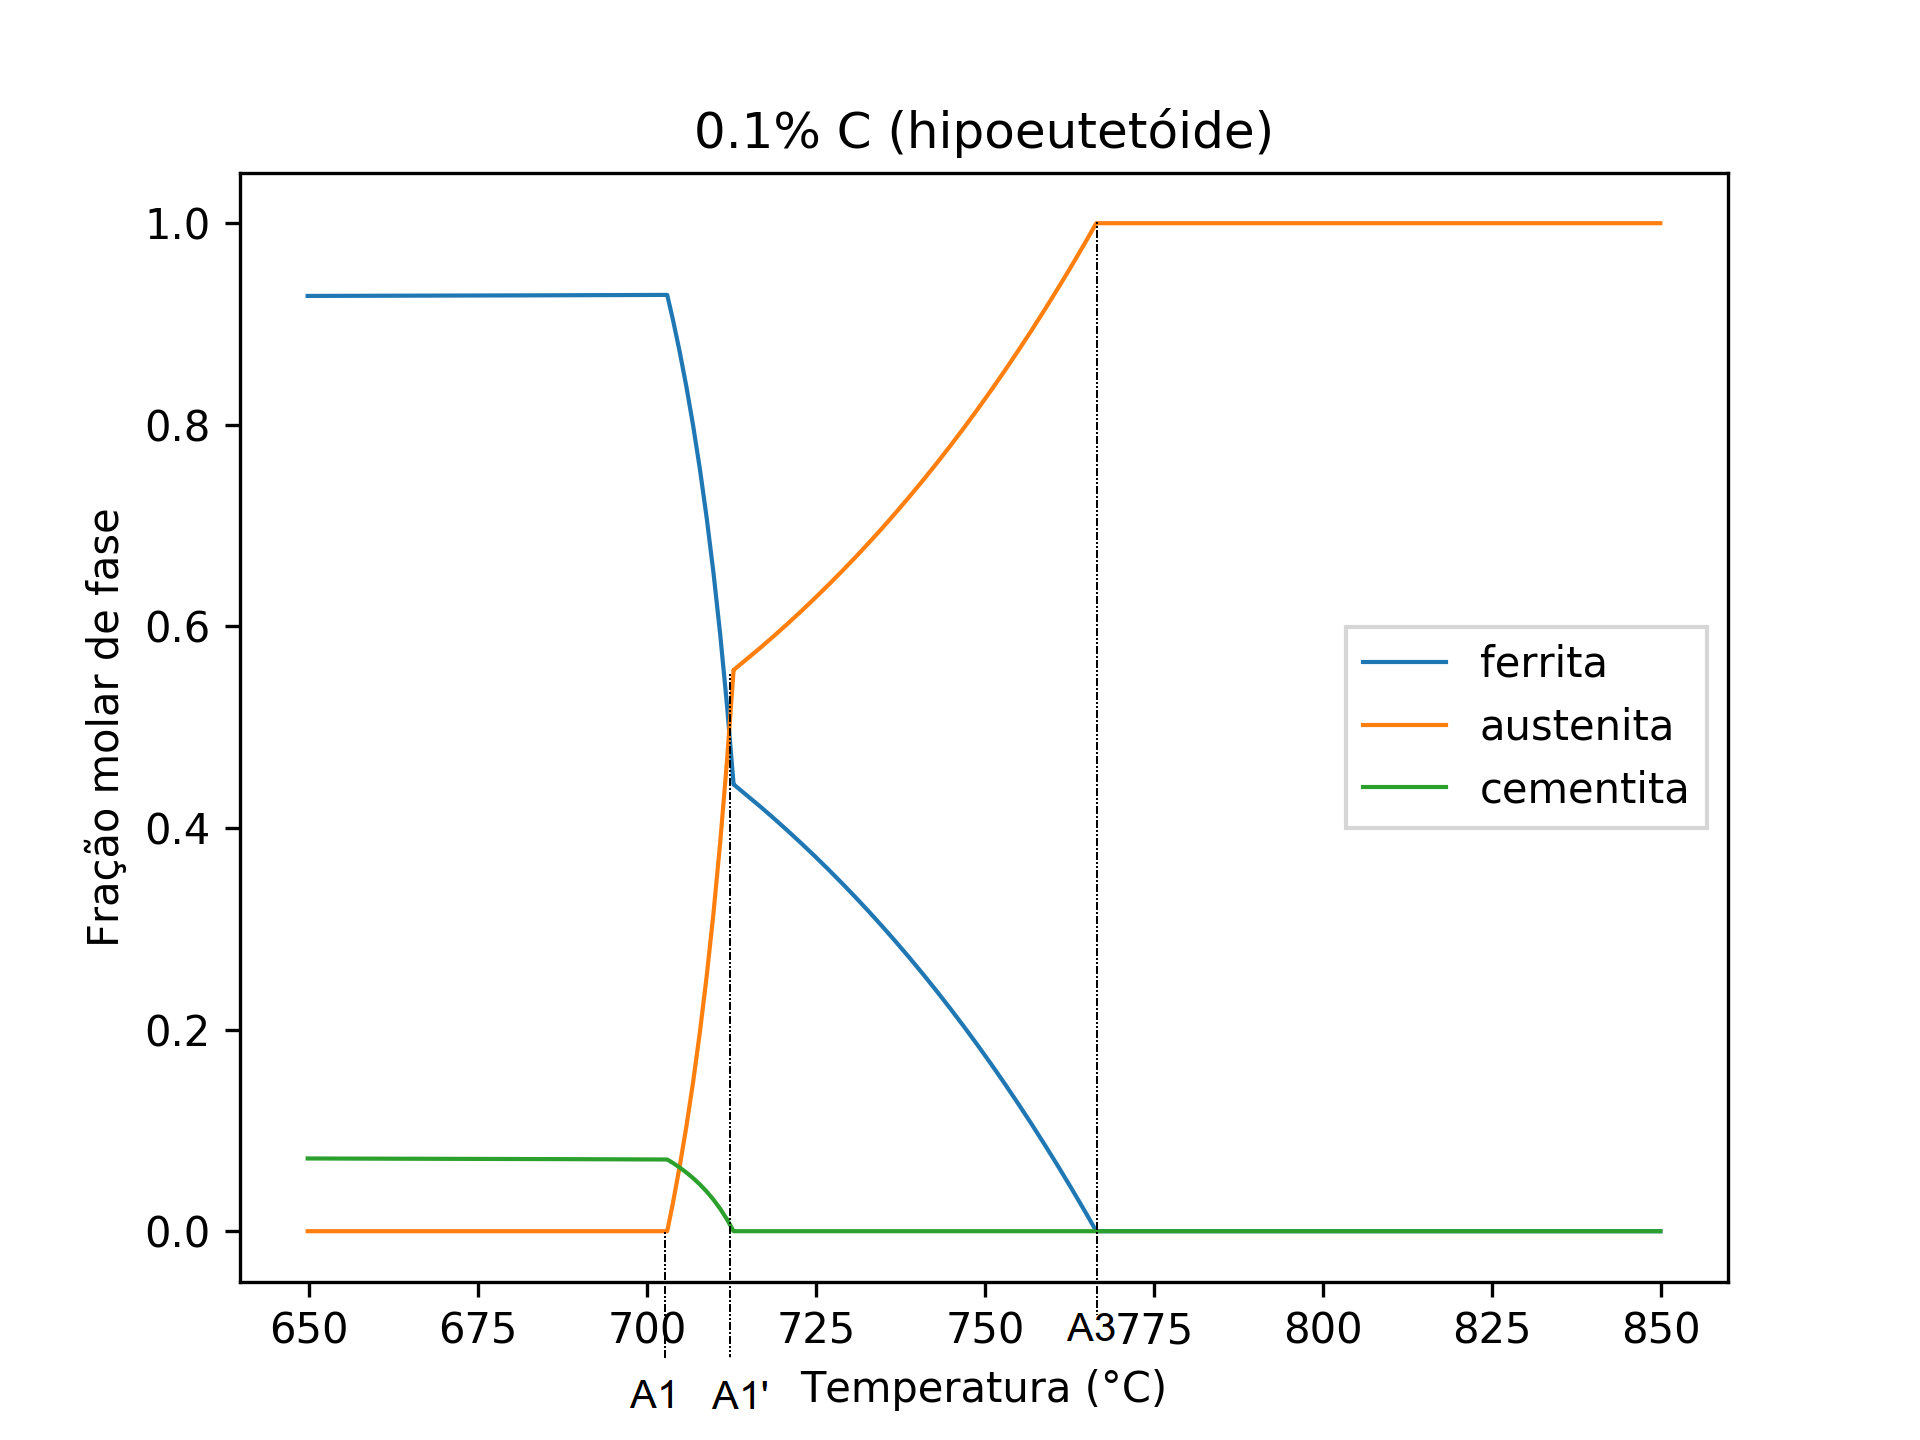
\includegraphics[width=.7\textwidth]{img/Fe-Mn-01C_edited.png}
  \caption{Fração molar de fase versus Temperatura para aço 0,1\%C 1\% Mn, em massa}
  \label{fig:fe-01c-1mn}
\end{figure}

Um aço nessa composição, mediante aquecimento, mantém as fases $\alpha$ e \ch{Fe3C} até chegar ao ponto A1, no qual a $\alpha$ começa a se decompor em $\gamma$. No gráfico da Figura \ref{fig:fe-01c-1mn}, esse ponto pode ser notado pela primeira mudança de inclinação da curva da austenita. O aço permanece no campo trifásico até encontrar o ponto A1', quando toda a fase \ch{Fe3C} se transforma em $\gamma$, a segunda mudança de inclinação na curva da austenita. Caso o aquecimento permaneça, a fase $\alpha$ começa a se transformar em $\gamma$, até atingir o ponto A3, onde tem-se 100\% de fase $\gamma$, a última mudança de inclinação na curva da austenita.

Um aço eutetoide, correspondente à segunda linha vertical tracejada da Figura \ref{fig:fe-1mn-C_isopleth} e ao gráfico da Figura \ref{fig:fe-0727c-1mn}, segue o mesmo raciocínio. A diferença é que não há um campo trifásico, por isso a temperatura A1' equivale à temperatura A3.

\begin{figure}[ht!]
  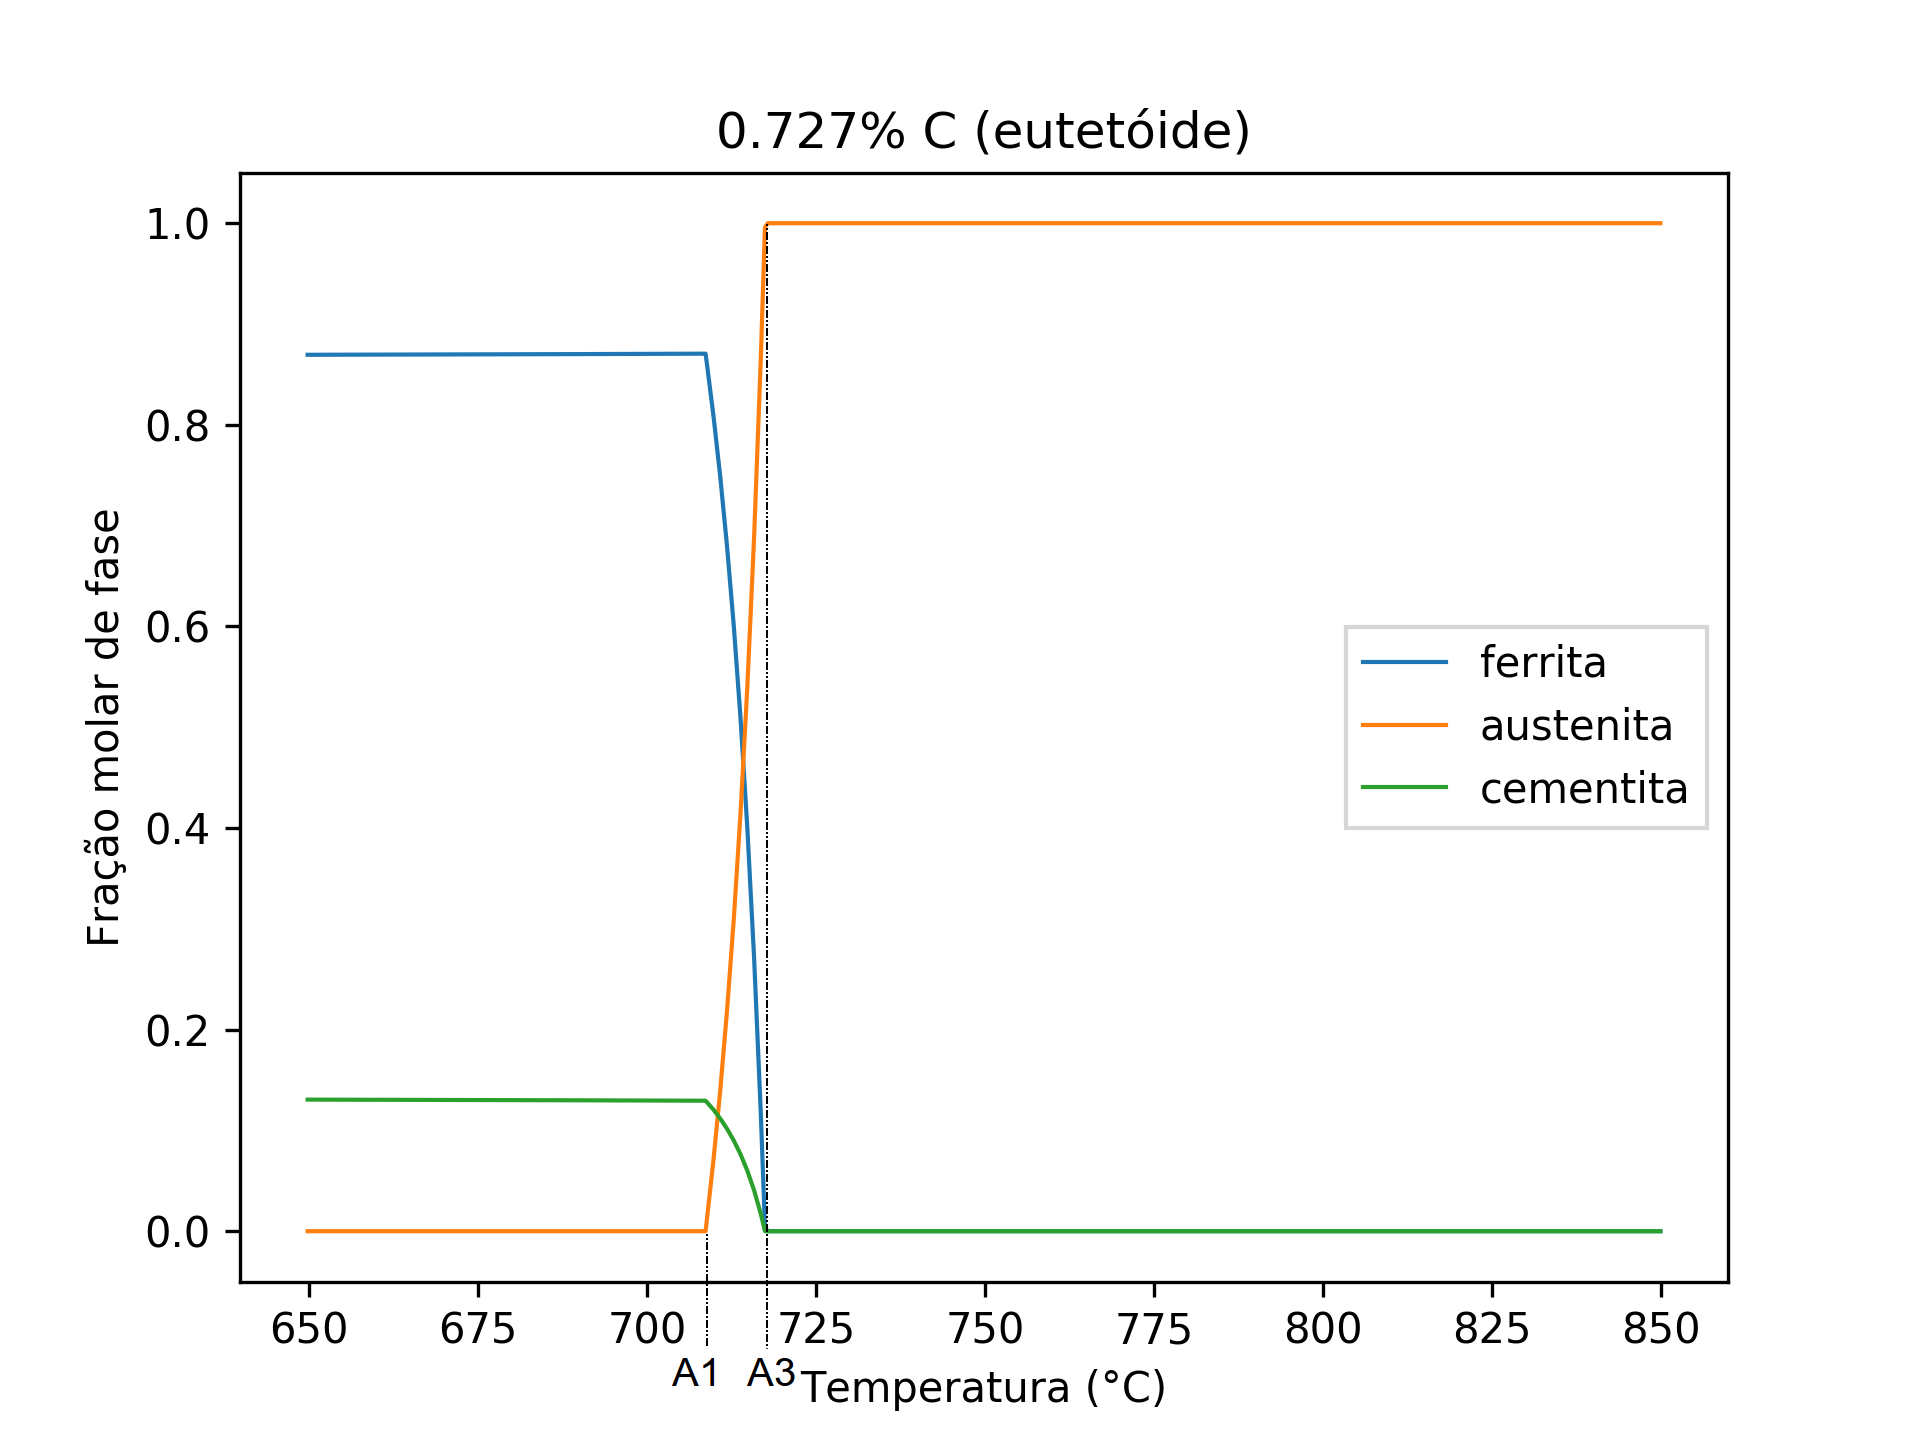
\includegraphics[width=.7\textwidth]{img/Fe-Mn-0727C_edited.png}
  \caption{Fração molar de fase versus Temperatura para aço 0,727\%C 1\% Mn, em massa}
  \label{fig:fe-0727c-1mn}
\end{figure}

Já para um aço hipereutetóide, terceira linha vertical tracejada da Figura \ref{fig:fe-1mn-C_isopleth} e gráfico da Figura \ref{fig:fe-1c-1mn}, a diferença é que o segundo campo bifásico é constituído por $\gamma$ e \ch{Fe3C}, até atingir o ponto em que toda a \ch{Fe3C} se transforma em $\gamma$. Certas literaturas, como \citet{Digges1960}, fazem distinção para a temperatura A3 de aços hipereutetóides, chamando-a de Acm, devido à diferença de campos bifásicos. No presente trabalho, ambas serão chamadas de A3, por corresponderem à mínima temperatura em que a fração de austenita é igual a um.

\begin{figure}[ht!]
  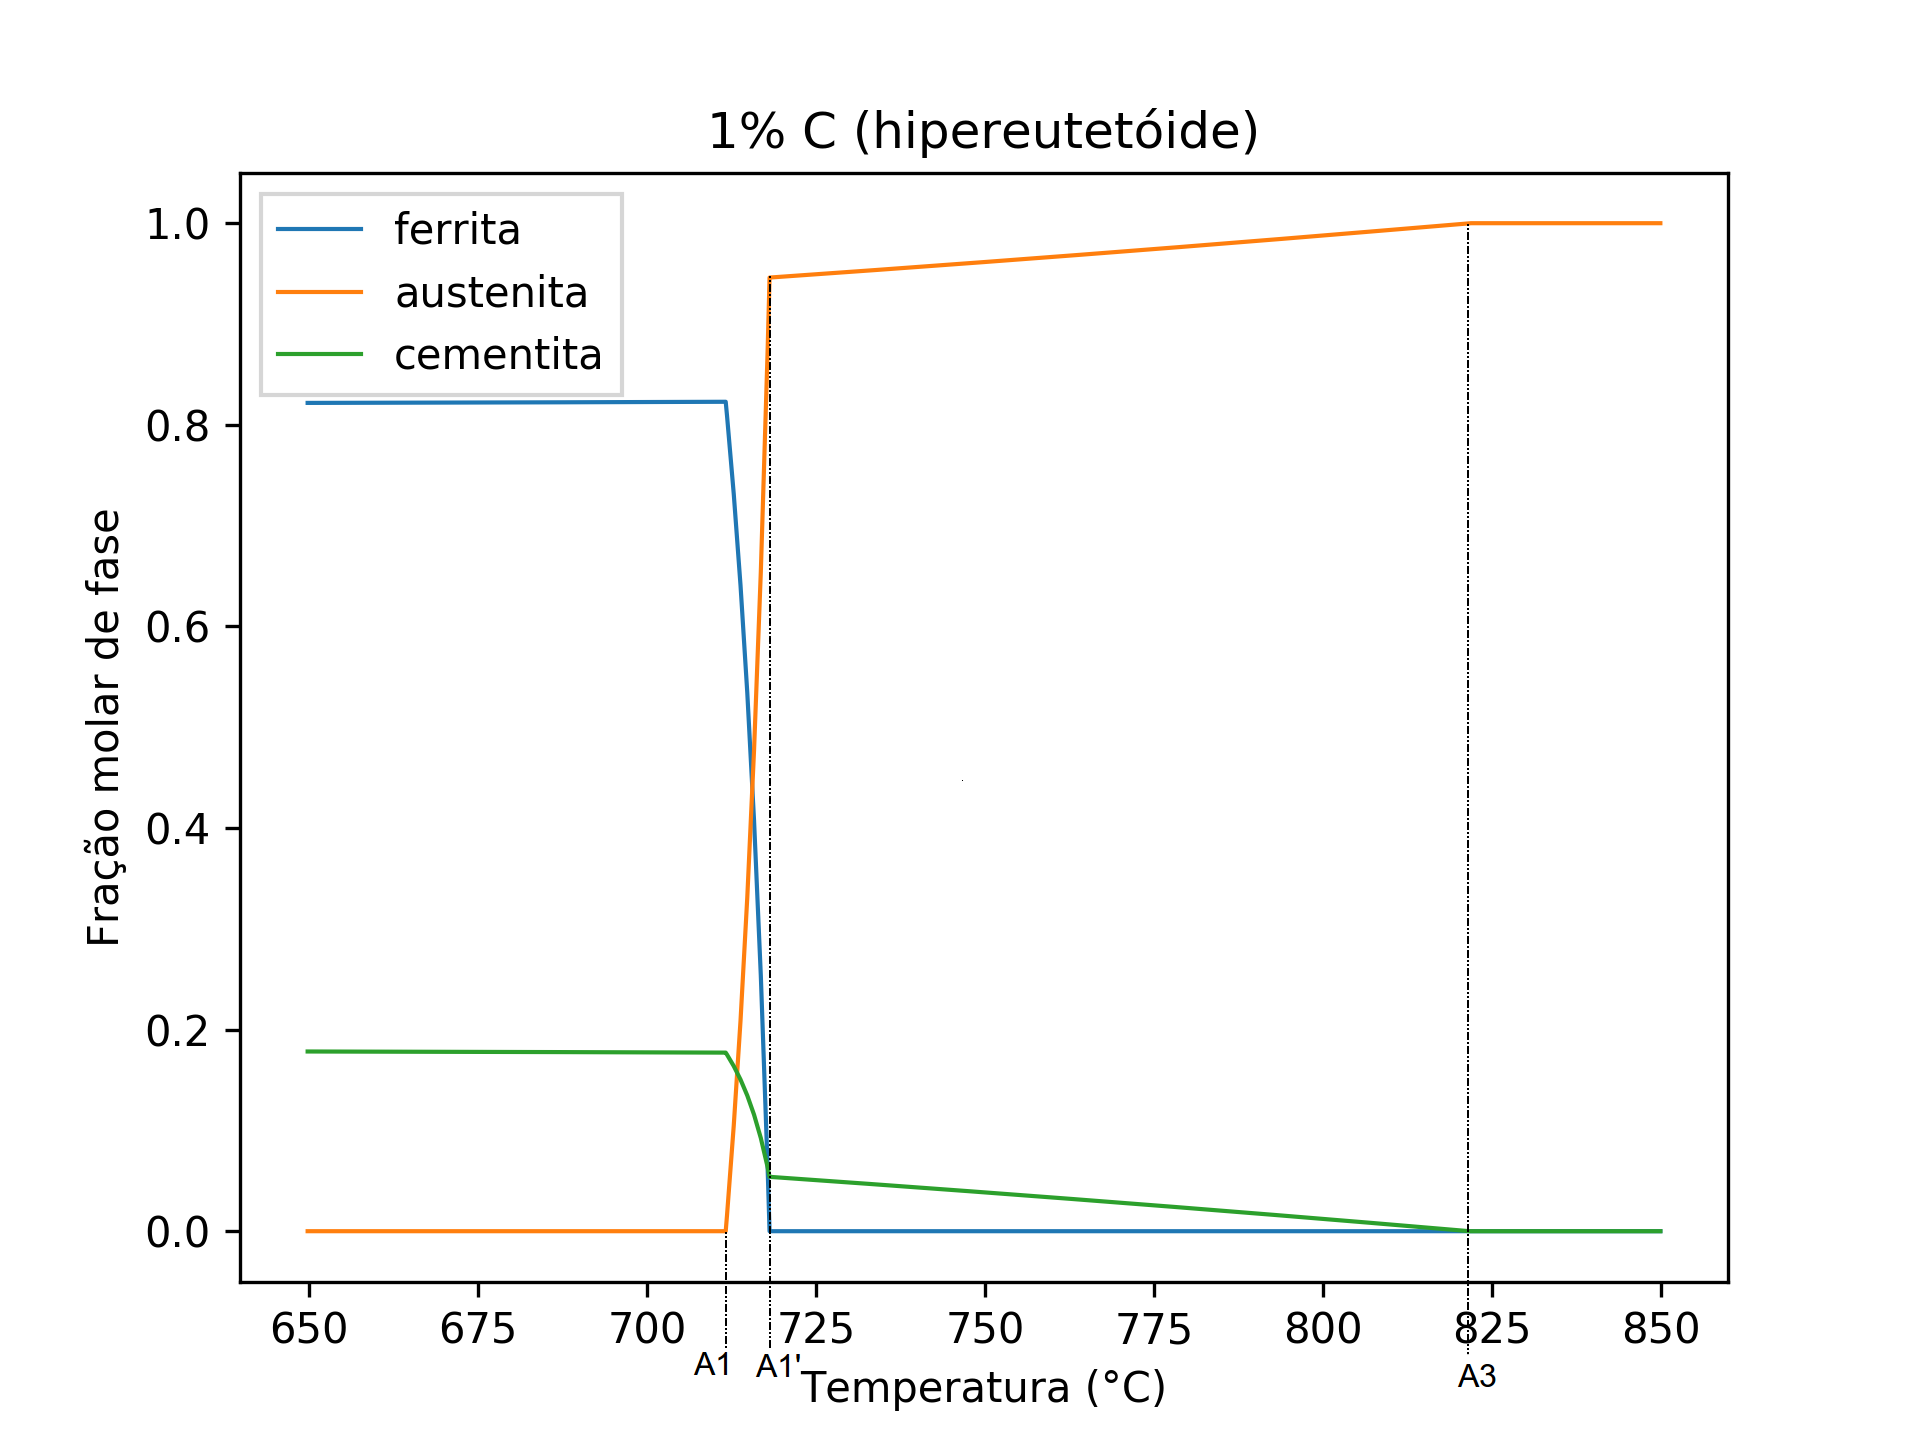
\includegraphics[width=.7\textwidth]{img/Fe-Mn-1C_edited.png}
  \caption{Fração molar de fase versus Temperatura para aço 1\%C 1\% Mn, em massa}
  \label{fig:fe-1c-1mn}
\end{figure}

Em resumo, a temperatura A1 corresponde à máxima temperatura em que a fração de austenita é zero. A3 é a mínima temperatura cuja fração de austenita é um. E A1' é o limite superior do campo intercrítico de três fases.

É possível ainda diferenciar a temperatura crítica no resfriamento da de aquecimento, utilizando respectivamente as letras ``r'' e ``e''. Em teoria, elas deveriam ser iguais, mas na prática a taxa de resfriamento ou aquecimento diferencia Ae1 de Ar1 e Ae3 de Ar3. A faixa de temperatura entre A1 e A3 é chamada de intervalo crítico ou de transformação \cite{Digges1960} \cite{Honeycombe1982}.

\section{Tratamento térmico de aços}

A obtenção das propriedades ideais de um aço está relacionada tanto com sua composição química quanto com os processos de tratamento térmico aos quais ele é submetido. Tratamentos térmicos podem ser utilizados para aumentar ou diminuir a ductilidade, dureza, tensão de escoamento ou tenacidade do material (TOTTEN, 2007).

A austenitização é a etapa que precede um tratamento térmico e consiste em aquecer o aço até a temperatura de formação da austenita. Esta pode ser parcial, quando se encontra na faixa de transformação, ou total, quando está acima do intervalo de transformação. A formação de uma estrutura cristalina cúbica de face centrada faz parte da normalização do aço \cite{ASM1991}.

A partir do aço na forma de austenita, é possível fazer o recozimento do aço, ou seja, o resfriamento lento para reduzir tensões, diminuir dureza para melhorar a usinabilidade, ajustar o tamanho do grão, reduzindo assim influências de tratamentos térmicos ou mecânicos anteriores. Para aços hipoeutetóides, os constituintes resultantes são perlita e ferrita, enquanto para hipereutetóides são cementita e perlita.

- Endurecimento

- Têmpera

\section{Determinação das Temperaturas Críticas}

- dilatometria

- computacionalmente: thermo calc

- eq empíricas (andrews)


\section{Aprendizado de m\'aquina e a determinação de Temperaturas Cr\'iticas}

Dada a complexidade e o custo de desenvolvimento de um novo material, estudos recentes têm se voltado para a tecnologia como primeira forma de avaliar hipóteses \cite{Belisle2015}. Uma vez que muitas variáveis estão envolvidas na determinação de uma propriedade, tornaram-se populares algoritmos capazes de aprender com alguma experiência vinda de um conjunto de tarefas,  cujo desempenho melhora quanto maior sua experiência, também chamados de machine learning ou aprendizado de máquina.

Esses algoritmos podem ser classificados entre supervisionados e não supervisionados. Ele é dito supervisionado quando recebe um banco de dados com as respostas certas e a partir delas prevê um valor para dada situação (regressão) ou faz uma classificação binária. Já o algoritmo não supervisionado não sabe quais são as respostas certas; ele é alimentado com dados para que se encontre um padrão (clusterização) (ANDREW, 200X).

No campo da engenharia de materiais, os algoritmos mais utilizados são os supervisionados, uma vez que pode-se reunir dados teóricos ou experimentais e a partir deles fazer a predição de propriedades. Diversas funções podem ser utilizadas para esse fim, cada uma com certa eficiência, e segundo o teorema ``No Free Lunch'' de Wolpert e Macready, não existe um algoritmo perfeito (apud BELISLE et. al.; 2015).

Dentre os métodos supervisionados, pode-se destacar alguns algoritmos. O primeiro e mais simples é a interpolação polinomial. Este pode se comportar de forma linear, como descrito na equação x, ou quadrática, como na equação y.

\begin{align}
  f(x) &= b x + c \\
  f(x) &= \frac{1}{2} a x^T + b x + c
\end{align}

Ambos são métodos muito utilizados devido ao baixo custo computacional. Entretanto, têm a necessidade de estabelecer alguma relação (linear ou quadrática) entre os termos estudados, utilizando termos fixos \cite{Bhadeshia1999}.

Um segundo método é a rede neural. Inspirada no cérebro humano, a rede neural baseia-se em associações para fazer previsões, sendo muito utilizada para reconhecimento de padrões. É indicada para funções não lineares e pode identificar relações complexas entre variáveis independentes. A desvantagem é o maior tempo computacional necessário \cite{Belisle2015}.

Uma rede neural tem uma camada de entrada, uma oculta e outra de saída. A camada de entrada recebe os dados e os envia para a camada intermediária, ou oculta, que os multiplica por um peso aleatório. A soma de todas as multiplicações é somada também a uma constante aleatória

\chapter{Metodologia}

\section{O Banco de Dados}

\label{sec:banco_dados}

A primeira etapa para elaboração de um algoritmo de machine learning é a construção do banco de dados utilizado em seu treinamento. Para este trabalho, utilizou-se dados extraídos do software Thermo-Calc\textregistered{}.

Inicialmente, discutiu-se os elementos de liga e suas respectivas faixas de composição química nos aços estudados. Foram considerados apenas os mais comuns aços de engenharia, cujas composições estão detalhadas na tabela x no apêndice bla. Não foram consideradas as composições relativas aos aços inoxidáveis. A Tabela xx mostra as faixas de composições escolhidas para criação do banco de dados de temperaturas críticas.

\begin{table}
  \caption{Faixas de composição química dos elementos de liga}

  \begin{tabular}{c c c}
  \hline
  \textbf{Elemento de liga} & \textbf{\% mínima} & \textbf{\% máxima} \\
  \hline
  Carbono & 0 & 1,5 \\
  Manganês & \SI{1e-6}{} & 3,0 \\
  Silício & \SI{1e-6}{} & 3,0 \\
  Cromo & \SI{1e-6}{} & 3,0 \\
  Níquel & \SI{1e-6}{} & 3,0 \\
  \hline
  \end{tabular}

  \label{tab:faixas_composicao}
\end{table}

Também discutiu-se a faixa de temperatura a ser estudada. Para isso, gerou-se diagramas binários para cada elemento de liga e observou-se suas temperaturas críticas.

Considerando a temperatura em que pode ser observada austenita, utilizou-se o intervalo de 673 a 1473K.

Definidas as faixas de composição química e temperatura, foram definidos os níveis para cada elemento, ou seja, quantas variações (ou steps) cada elemento tem. O valor do step é dado pela equação a seguir.

\begin{equation}
  step = \frac{\Delta c}{n - 1}
\end{equation}

Assim, os níveis e steps utilizados para cada elemento são dados na tabela a seguir.

\begin{table}
  \caption{Níveis e steps para cada elemento de liga}

  \begin{tabular}{c c c}
  \hline
  \textbf{Elemento de liga} & \textbf{Níveis} & \textbf{Valor do step} \\
  \hline
  Carbono & 11 & 0,15 \\
  Manganês & 5 & 0,75 \\
  Silício & 5 & 0,75 \\
  Cromo & 5 & 0,75 \\
  Níquel & 5 & 0,75 \\
  \hline
  \end{tabular}

  \label{tab:faixas_composicao}
\end{table}


Já para a temperatura, estabeleceu-se um step de 10K. A partir da combinação desses valores de composição, um script faz a chamada do Thermo-Calc\textregistered{}. Dessa forma, para dada composição química, são retornadas as porcentagens de cada fase (ferrita, austenita e cementita) para cada temperatura dentro da faixa estabelecida.

O resultado da chamada do Thermo-Calc\textregistered{} é salvo em um arquivo .DAT. No total, foram gerados 6874 arquivos.

\section{Extra\c{c}\~ao de temperaturas cr\'iticas}

Para cada arquivo gerado pela chamada do Thermo-Calc\textregistered{}, calculou-se as temperaturas críticas através de outro script. Este faz a leitura do arquivo .DAT, que contém as porcentagens de cada fase para cada temperatura entre 673 e 1473K, variando em 10K.

Para determinar a A1, identifica-se a maior temperatura em que a porcentagem de austenita é zero, enquanto para o A3, identifica-se a menor temperatura em que a porcentagem de austenita é um.

Também identificou-se a temperatura crítica intermediária, A1', e consequentemente se o aço do respectivo arquivo é hipo ou hipereutetóide. Para isso, comparou-se a temperatura em que a porcentagem de ferrita é zero ($T_{ferr}$) com a que a porcentagem de cementita é zero ($T_{cem}$). Caso $T_{ferr}$ seja maior que $T_{cem}$, A1' é igual a $T_{cem}$ e o aço é hipoeutetóide; caso contrário, A1' é igual a $T_{ferr}$ e o aço é hipereutetóide. A terceira hipótese é que não houvesse cementita para a composição dada, assim não haveria campo trifásico e A1' seria igual a A1.

Os dados do nome do arquivo, o número da macro que fez sua chamada, composição química, temperaturas críticas e classificação em hipo ou hiper eutetóide foram salvos em um arquivo CSV.

\section{Experimentos}

Foram realizados testes para averiguar a qualidade dos dados extraídos do Thermo-Calc\textregistered{}.

Para avaliar a coerência, foi elaborado um script que plota simultaneamente o gráfico da porcentagem de austenita em função da temperatura, comparando dados da tabela de resultado com dados de uma única chamada do Thermo-Calc\textregistered{}. Dessa forma, foi possível testar resultados pontuais considerados inconsistentes.

Outro teste para averiguar os dados foi a verificação da existência das fases ferrita, austenita e cementita.

Uma importante verificação da base de dados como um todo foi a comparação com os resultados das equações empíricas de Andrews. Para cada composição química do banco de dados, calculou-se as temperaturas críticas A1 e A3 pelas equações empíricas. A partir disso, gerou-se um gráfico de temperatura crítica calculada versus temperatura crítica gerada pelo Thermo-Calc\textregistered{}.

A fim de avaliar o efeito de cada elemento na temperatura crítica A3, foram traçadas isopletas com a composição de carbono como variável livre e diferentes composições de cada elemento.


\chapter{Resultados e discussão}

O resultado da variação de composição química para aços carbono gerou um total de 6874 combinações e, para cada, fez-se a chamada do Thermo-Calc\textregistered{} que retorna a porcentagem de cada fase para temperaturas de 673 a 1473K, variando de 10K. Para cada composição, os dados são salvos em um arquivo .DAT.

Inicialmente, sete macros faziam a chamada do Thermo-Calc\textregistered{} com 1000 composições cada. Isso trouxe resultados muito inconsistentes, como valores em branco ou ou incoerentes com a literatura, e podem estar relacionados ao num sei. Notou-se que, quanto menos chamadas cada macro fazia, menor o número de erros nos resultados e, assim, chegou-se ao número de 69 macros com 100 chamadas cada.

Em seguida, para cada arquivo, extraiu-se as temperaturas críticas A1, A1' e A3. As imagens a seguir ilustram a lógica dessa extração.

\begin{figure}
  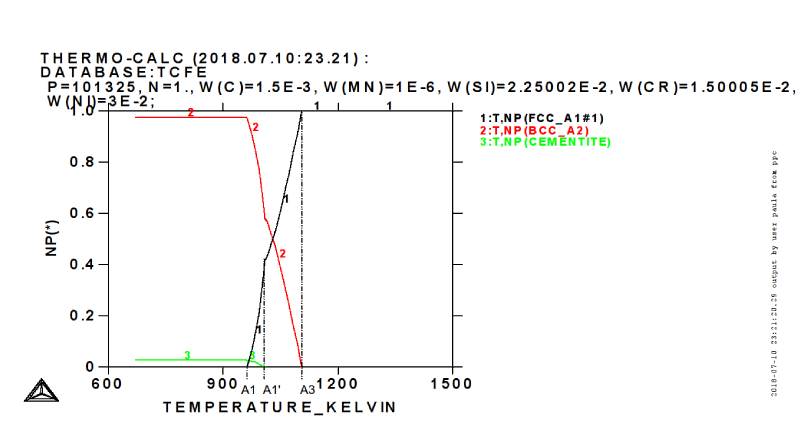
\includegraphics[width=.9\textwidth]{img/714editado.png}
  \caption{Extração de temperaturas críticas para aço hipoeutetóide}
  \label{fig:Tcrit_liga_hipo}
\end{figure}

\begin{figure}
  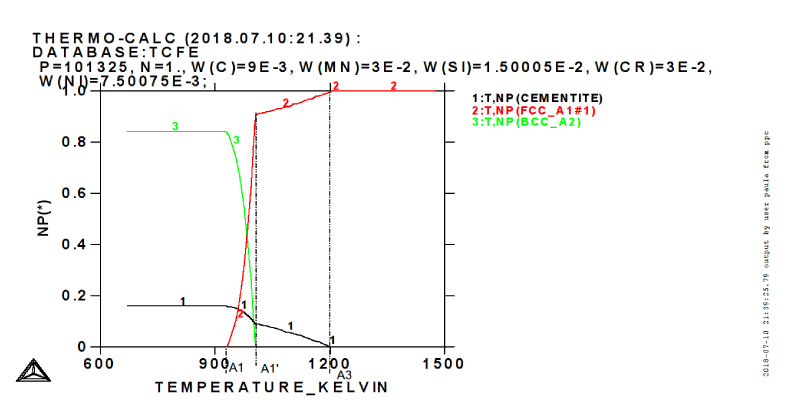
\includegraphics[width=.9\textwidth]{img/4321editado.png}
  \caption{Extração de temperaturas críticas para aço hipereutetóide}
  \label{fig:Tcrit_liga_hiper}
\end{figure}

\begin{figure}
  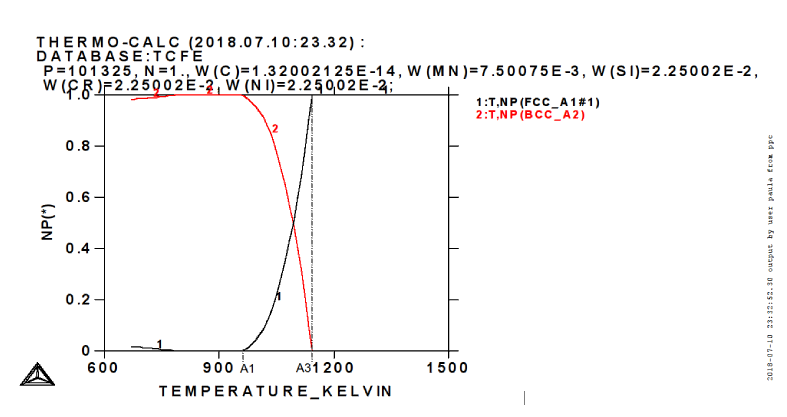
\includegraphics[width=.9\textwidth]{img/418editado.png}
  \caption{Extração de temperaturas críticas para aço hipoeutetóide sem cementita}
  \label{fig:Tcrit_liga_sem_cementita}
\end{figure}

A temperatura A1' é representada pela mudança de inclinação na curva da porcentagem de austenita. Para aços hipoeutetóides, essa temperatura corresponde ao ponto em que a porcentagem de cementita é zero, como mostra a figura x. Já para hipereutetóides, ao ponto em que a porcentagem de ferrita é zero, como na figura x. Enquanto isso, para aços em que a porcentagem de cementita é sempre zero, considera-se que a temperatura A1' é igual à A1.

É importante destacar que nem sempre um aço terá as três temperaturas críticas. Elementos muito alfagênicos podem não ter A3, como no caso de um $\gamma$ loop, e gamagênicos podem não ter A1, por terem austenita estável à temperatura ambiente.

Mesmo considerando que algumas temperaturas críticas podem não existir para certas composições, ainda está em estudo os erros que ocorreram nessa extração. Por exemplo, algumas composições com baixo carbono ficaram com valores em branco, enquanto outras tiveram valores de temperatura crítica muito acima do esperado, embora os gráficos plotados para sua respectiva composição estivesse dentro do esperado. Pretende-se corrigir esses erros antes dos resultados serem utilizados em um algoritmos de machine learning.
Também foi realizada uma comparação dos valores de temperatura crítica com a equação empírica de Andrews, plotando o gráfico da figura x. A linha em azul representa os valores esperados ($T_{empirical} = T_{database}$).

Figura: Gráfico de temperatura crítica calculada pela equação empírica de Andrews e temperatura crítica do banco de dados

Nota-se que, para as temperaturas A3, existe uma correlação maior com os valores calculados pela equação empírica, enquanto para A1 existe uma divergência maior. Isso pode estar relacionado a erros no script que extrai a temperatura A1, que ainda está em revisão. Outro fator que influencia na divergência é o fato de a equação de Andrews não ter membros interdependentes entre os elementos químicos, o que na prática não se aplica.

Para averiguar essa interdependência, plotou-se as isopletas de temperatura para cada elemento, variando a composição de carbono. Para cada elemento de liga, plotou-se cinco curvas, correspondentes aos cinco níveis de composição escolhidos.

Para o manganês e níquel, nota-se que a baixas concentrações de carbono a concentração do elemento de liga tem muita interferência no valor das temperaturas de transformação. A partir de 0,8\% C, as temperaturas são mais próximas para todos os níveis. Uma possível explicação é que os três elementos são gamagênicos.

Já para elementos alfagênicos, como o cromo, a relação se inverte. Para baixas concentrações de carbono, os valores de temperatura ficam próximos, e a partir de 0,4\% de carbono a concentração do cromo já contribui para sua divergência.

Um caso intermediário é o do silício, que apesar de alfagênico, tem influência na temperatura tanto a baixas quanto a mais altas concentrações de carbono, embora a influência a baixas concentrações seja maior.

\chapter{Conclusões parciais}

\bibliography{/home/paula/Documentos/TCC/artigos/tcc.bib}

\end{document}
